\documentclass{article}
\usepackage{arxiv}
\usepackage{authblk}
\usepackage[utf8]{inputenc}
\usepackage[T1]{fontenc}
\usepackage{amsmath,amssymb,amsthm,mathtools}
\usepackage{microtype}
\usepackage{booktabs,tabularx,array,graphicx}
\usepackage[authoryear,round]{natbib}
\usepackage{needspace,placeins}
\usepackage{xcolor}
\usepackage[mathlines]{lineno}
\usepackage[colorlinks=true,allcolors=black]{hyperref}
\usepackage{bookmark}
\urlstyle{same}
\pagecolor{white}
\color{black}
\renewcommand{\linenumberfont}{\normalfont\sffamily\scriptsize}

\numberwithin{equation}{section}
\newcounter{algorithm}
\newtheorem{theorem}{Theorem}[section]
\newtheorem{proposition}[theorem]{Proposition}
\newtheorem{lemma}[theorem]{Lemma}
\newtheorem{corollary}[theorem]{Corollary}
\theoremstyle{remark}
\newtheorem{remark}[theorem]{Remark}
\newtheorem*{precisionremark}{Remark}
\newcommand{\E}{\mathbb E}
\newcommand{\R}{\mathbb R}
\newcommand{\one}{\mathbf 1}
\newcommand{\norm}[1]{\lVert#1\rVert}
\DeclareMathOperator{\Var}{Var}
\DeclareMathOperator{\Cov}{Cov}
\DeclareMathOperator{\tr}{tr}
\DeclareMathOperator{\diag}{diag}
\DeclareMathOperator{\ESS}{ESS}
\setlength{\emergencystretch}{2em}

\title{Certified Approximation of Cover's Universal Portfolio}
\author[1, 2]{James Chok}
\author[ ]{Domenic Petzinna}
\affil[1]{School of Mathematics and Maxwell Institute for
  Mathematical Sciences, University of Edinburgh, United Kingdom}
\affil[2]{School of Mathematics and Statistics, UNSW Sydney,
  Australia}

\date{November 2026}
% \renewcommand{\headeright}{Working draft}
% \renewcommand{\undertitle}{Working draft}

\renewcommand{\shorttitle}{Certified Approximation of Cover's Universal Portfolio}
\hypersetup{
  pdftitle={Certified Approximation of Cover's Universal Portfolio},
  pdfauthor={James Chok and Domenic Petzinna},
  pdfsubject={Certified benchmark wealth and anytime-valid inference},
  pdfkeywords={universal portfolios, online portfolio selection, Dirichlet moments, interval arithmetic, e-values, anytime-valid inference, benchmarks}
}
\bibliographystyle{plainnat}

\begin{document}
\maketitle
\raggedbottom
\linenumbers

\begin{abstract}
Cover's universal portfolio earns the prior average of the wealth of all
constant-rebalanced portfolios, so comparing another strategy with Cover
requires evaluating an integral over portfolio weights. For any symmetric
Dirichlet prior, we construct an outward-rounded interval for the difference
between Cover's log wealth and that of a strategy with positive payoffs.
We integrate the linear part of log wealth by exponential tilting and bound
the remaining curvature using Dirichlet moment series, retaining days with
zero price relatives as exact polynomial factors. Since only the returns and
the prior enter this calculation, the same enclosure can be used to compare
every strategy on a given return history. On 50 stocks over 26 years, the
certified wealth band was at most 0.062 percentage points wide relative to an
independent reference. On four of six standard benchmarks, we certified that
an $O(d)$ first-order update tracked Cover to within $10^{-4}$ in log wealth
at every close, with a smaller measured peak error than any of the
100,000-portfolio Monte Carlo replays we tested. Published universal-portfolio
wealths differed from the certified midpoints by up to 1.6\%, and on NYSE(N)
using the toolbox approximation in place of Cover reversed its ranking
relative to equal weighting (1/N). The lower endpoint also gives an anytime-valid
test of whether 1/N is growth-optimal. None of the eight observed markets
crossed the rejection threshold, and an experiment with a planted persistent
advantage illustrates how averaging over losing portfolios can delay detection
for decades.
\end{abstract}
\keywords{universal portfolios \and online portfolio selection \and
  Dirichlet moments \and interval arithmetic \and e-values \and anytime-valid inference \and benchmarks}

\section{Introduction}
Consider an investor trading $d$ stocks over a fixed horizon $T$. If
$C_{t,i}$ denotes the closing price of stock $i$ on day $t$, then
$x_{t,i}=C_{t,i}/C_{t-1,i}$ is its price relative for that day,
$1\le t\le T$. At close $t-1$ the investor chooses an allocation
$w_t\in\mathcal S_d:=\{w\in\mathbb{R}^d:\sum_i w_i=1,\ w_i\ge0\}$,
where $w_{t,i}$ is the fraction of wealth held in stock $i$ until the next
close. An initial investment of one dollar therefore grows to
\begin{equation}
  V_T=\prod_{t=1}^T(w_t\cdot x_t).
\end{equation}

The investor would like to choose $\{w_t\}_{t=1}^T$ to maximize $V_T$,
but must choose $w_t$ before observing $x_t$. To evaluate such a strategy,
we compare its wealth with that of the best constant-rebalanced portfolio
in hindsight. A portfolio that restores the same weights $w$ each day
earns $S_t(w)$ by close $t$, giving the log regret
\begin{equation}
  R_T(V)=\max_{w\in\mathcal S_d}\log S_T(w)-\log V_T,\qquad
  S_t(w)=\prod_{s=1}^t(w\cdot x_s).
\end{equation}
Thus, when $R_T(V)/T\to0$, the difference in average log growth per trading
day between the strategy and its hindsight benchmark tends to zero.

\citet{cover1991} introduced the universal portfolio to achieve this
property. In the formulation of \citet[Definition~1]{coverordentlich1996},
a prior $\pi$ on the simplex $\mathcal S_d$ determines the initial
distribution of capital among the fixed portfolios. After $t$ days the
capital assigned to each portfolio has grown in
proportion to its wealth $S_t(w)$, so the aggregate allocation for the
next day is
\begin{equation}
  w_{t+1}^\mathrm{Cover} = \frac{\int_{\mathcal S_d} w S_t(w)\,\pi(dw)}{Z_t},
 \qquad Z_t=\int_{\mathcal S_d}S_t(w)\,\pi(dw).
\end{equation}
The normalizing integral $Z_t$ also gives Cover's wealth. Indeed, the
one-day payoff is the ratio of successive integrals, so with $Z_0=1$ the
product of these payoffs telescopes,
\begin{equation}
  V_t^\mathrm{Cover} = \prod_{s=1}^t(w_s^\mathrm{Cover}\cdot x_s)=\prod_{s=1}^t\frac{Z_{s}}{Z_{s-1}}=Z_t.
\end{equation}
With the uniform prior, Cover's regret is at most $(d-1)\log(T+1)$ on
every return sequence \citep[Theorem~1]{coverordentlich1996}, and for
fixed $d$ this is the optimal worst-case order in $T$
\citep{ordentlichcover1998}. The difficulty in implementing the
strategy lies in computing $Z_t$. Direct expansion of $S_t(w)$ produces
$\binom{t+d-1}{d-1}$ coefficients in the dense case, making the exact
recursion expensive as the number of stocks grows
\citep{coverordentlich1996}.

Several online portfolio strategies compute their allocations without
evaluating Cover's integral
\citep{helmbold1998,agarwal2006,hazankale2015,gaivoronskistella2000}.
\citet{chokvasil2025} develop the Cauchy--Simplex algorithm for convex
optimization on the simplex and apply it to portfolio selection.
The VB-FTRL strategy of
\citet{jezequel2026} achieves the same logarithmic order of regret with an
efficient update. This guarantee controls the loss relative to the best fixed
portfolio in hindsight, leaving open how closely VB-FTRL tracks Cover on a
particular return history.

A numerical implementation of Cover faces a question on each trading
date: how much of the reported wealth difference could be integration
error? In the spirit of the Solvability Complexity Index programme's
work on certified spectral computation
\citep{benartzi2020computing,colbrookhansen2023foundations,chokcolbrook2026},
we compute a finite-precision interval guaranteed to contain
$\log Z_t$. Subtracting the log wealth of the allocations actually
played gives an \emph{a posteriori} bound on
$\Delta_t=\log Z_t-\log V_t$. We require nonnegative price relatives
with at least one positive entry per day, and positive payoffs for the
strategy whose log wealth we compare.

The 23-stock NYSE(N) benchmark \citep{li2014survey,li2016olps} illustrates
why the integration error matters. In our replay from 1985 to 2010, one
dollar invested in the OLPS toolbox's universal portfolio grew to \$31.558,
just ahead of the \$31.552 earned by the equal-weight strategy (1/N). Our certificate places Cover's
terminal wealth between \$31.00 and \$31.25, rounded outward, thus establishing
that Cover finished $0.96$--$1.73\%$ behind 1/N. On this benchmark the toolbox
replay overstated Cover's wealth by $0.99$--$1.78\%$, enough to reverse the
ranking of the two portfolios (Section~\ref{sec:audit}).

\Needspace{5\baselineskip}
\paragraph{Contributions.}
\begin{enumerate}
\item We derive explicit endpoints for $\Delta_t$ under any symmetric
Dirichlet prior (Theorem~\ref{thm:main}). A product tilt accounts exactly for days with zero price
relatives, while positive moment series and outward rounding give computable
bounds for the remaining integrals
(Section~\ref{sec:certificate}).
\item On six standard OLPS datasets we use the same enclosure to compare
Cover with a first-order update, sampled universal portfolios, Soft-Bayes
and VB-FTRL. This also allows us to audit published universal-portfolio
wealths, after which we examine the cost of computing the enclosure on
panels of up to 403 assets (Section~\ref{sec:bench}).
\item We use the lower endpoint to test whether 1/N is growth-optimal,
allowing the observer to stop at any close. Using eight market histories,
a planted advantage and 2,026 stock subsets, we examine when a realized
wealth advantage over 1/N provides statistical evidence against its growth
optimality (Section~\ref{sec:test}).
\end{enumerate}

\paragraph{Computing Cover's integral.}
\citet{coverordentlich1996} give an exact coefficient recursion for Cover's
wealth and study the choice of Dirichlet prior. Since the integrand is a
product of linear forms, the same integration problem arises in queueing
models \citep{casale2017} and is closely related to exact methods for
integrating polynomials on a simplex and evaluating marginal likelihoods
\citep{baldoni2011,lin2009}. One alternative to exact integration is to
sample fixed portfolios, as analyzed by \citet{blumkalai1999}, who also
consider transaction costs. \citet{kalai2002} give a sampling algorithm and
identify return histories on which sampling directly from the prior is
expensive. For more general families of strategies, \citet{akcoglu2004}
study probabilistic approximation, while \citet{crossbarron2003} obtain
closed-form updates for particular classes of past-dependent targets.

\paragraph{Efficient strategies and regret.}
Exponentiated Gradient, Soft-Bayes, Ada-BARRONS and Damped Online Newton
Step all use a hindsight portfolio as the benchmark for the trader's log
wealth \citep{helmbold1998,orseau2017,luo2018,mhammedi2022}.
\citet{vanerven2020} asked whether plain log-barrier FTRL could achieve
$O(d\log T)$ regret without a uniform gradient bound. \citet{zimmert2022}
disproved the conjectured dependence on dimension and obtained
polylogarithmic regret with BISONS. By adding a volumetric barrier,
VB-FTRL achieves regret at most $564d\log(T+560d)$ at a per-round cost of
$\widetilde O(d^2(T+d))$ \citep[Theorem~4.1 of the preprint]{jezequel2026}.
Regret bounds also have statistical applications, as illustrated by the
confidence sequences obtained from the two-asset half-Dirichlet portfolio
\citep{orabona2024}.

\paragraph{Benchmarks for online portfolio selection.}
We draw on the benchmark strategies surveyed by \citet{li2014survey} and
on the OLPS toolbox, which distributes six daily return matrices together
with a random-walk approximation to the universal portfolio
\citep{li2016olps}. The higher-dimensional NYSE(N) and SP500 panels
provided by FinOL allow us to study how the cost grows with the number
of assets \citep{finol}. We also compare Cover with 1/N, which \citet{demiguel2009optimal}
found difficult to outperform out of sample using estimated portfolios.

\paragraph{Testing by betting.}
A nonnegative martingale starting at one reaches $1/\delta$ with probability
at most $\delta$ \citep{ville1939}. Consequently, when discounted wealth
is a martingale under the null, a trading strategy gives a test that may be
monitored at every close \citep{shafer2019game,ramdas2023game}.
\citet{vovk2011efficient} and \citet{vovk2016probabilityfree} study market
efficiency through the extent to which a strategy can outperform an index,
and \citet{takeuchi2011new} use betting strategies to test martingale
hypotheses for stock prices. In the benchmark approach, assets measured in
units of the num\'eraire portfolio have nonpositive conditional drift, and
under diversification assumptions 1/N can approximate this portfolio as
the market grows \citep{platen2012approximating}. Universal-portfolio
mixtures have also been used to construct confidence sequences
\citep{orabona2024,ryu2024gambling}. Here we take 1/N as the index and
Cover's portfolio as the bet, using the certified lower endpoint to implement
the test even when exact integration of the mixture is impractical.

\paragraph{Verified numerics.}
We use scrambled net quadrature to obtain an independent numerical estimate
of Cover's wealth \citep{owen1997}. To certify the wealth difference, we
enclose the integral analytically, bound the truncation error and evaluate
the resulting expressions in Arb with outward rounding
\citep{rump2010,johansson2017arb}. The certificate therefore remains valid
regardless of the accuracy of the quadrature estimate.

\section{Cover wealth and a first-order portfolio}
\label{sec:setup}

Let $W\sim\pi=\operatorname{Dirichlet}(\alpha\one)$ be a portfolio on the
simplex of $d\ge2$ assets, where $\alpha>0$ and the uniform prior
($\alpha=1$) is used unless stated otherwise. We assume that each return
vector $x_s$ is nonnegative and has at least one positive entry. For a
strategy with positive daily payoffs, we measure the discrepancy from
Cover at the close of day $t$ by the signed log-wealth error
\begin{equation}
  \Delta_t=\log Z_t-\log V_t .
  \label{eq:fidelity}
\end{equation}

To remove the common market return, we divide each row by the equal-weight
payoff $\bar x_s=u^\top x_s$, where $u=\one/d$. This normalization
preserves the ratio of the two wealths and places each asset return in
$[0,d]$, allowing us to work with the centered returns
\[
 a_s=x_s/\bar x_s-\one,\qquad g_0=0,\qquad
 g_t=\sum_{s=1}^t a_s,\qquad y_s=a_s^\top W .
\]
Each $a_s$ thus has coordinate sum zero, and a fixed portfolio earns the
normalized payoff $1+y_s$, which is positive almost surely under the
Dirichlet prior. Its normalized log wealth is consequently
$F_t=\sum_{s=1}^t\log(1+y_s)$, so the normalized wealths
$\bar Z_t=\E e^{F_t}$ and $\bar V_t=V_t/\prod_{s=1}^t\bar x_s$ have the
same signed log difference as the original wealths.

To obtain a first-order portfolio, we retain the term in $e^{F_t}$ that is
linear in the centered returns, namely $g_t^\top W$. Since $\E W=u$ and
$g_t^\top u=0$, the corresponding approximation to Cover's next allocation is
\[
 \frac{\E[We^{F_t}]}{\E e^{F_t}}
 \ \simeq\ u+\Cov(W)g_t,\qquad
 \Cov(W)=\frac{I-\one\one^\top/d}{d(d\alpha+1)} .
\]
The resulting predictable portfolio, which takes $O(d)$ operations to
update on rounds when its allocation lies in the interior of the simplex, is
\begin{equation}
 w_s^{\mathrm{FO}}=u+\frac{g_{s-1}}{d(d\alpha+1)} .
 \label{eq:first-order}
\end{equation}
Nonnegativity of the price relatives gives the upper bound $x_{s,i}/\bar x_s\le d$.
The usual no-junk-bond condition also imposes a lower bound, requiring
every ratio $x_{s,i}/\max_j x_{s,j}$ to be at least a common $a>0$
\citep[Remark~12 and Theorem~13]{chokvasil2025}. Our certificate allows
$a=0$, since a zero gross return wipes out the investment in that stock
while the equal-weight payoff and Cover wealth remain positive whenever
another stock has a positive gross return. In this setting the log-loss
gradient $-x_s/(w^\top x_s)$ can be unbounded as $w$ approaches a face of
the simplex, as emphasized by \citet{vanerven2020}.

\begin{remark}[Why first order can track wealth closely]
Consider a fixed horizon and scale every centered return by a common factor
$h\to0$. Writing $G=\sum_s y_s$, $Q=\sum_s y_s^2$, and
$c_s=a_s^\top g_{s-1}/[d(d\alpha+1)]$, we obtain $1+c_s$ as the
normalized payoff of \eqref{eq:first-order}. Expanding
$\|g_s\|^2-\|g_{s-1}\|^2$ and using the covariance above gives
$\sum_s c_s=(\E G^2-\E Q)/2$, which is precisely the quadratic term
of $\E\prod_s(1+y_s)$. The two wealths therefore agree through second
order, giving $\log\bar Z_t-\log\bar V_t^{\mathrm{FO}}=O(h^3)$ at
fixed $t$. In particular, $\E G^2=\|g_t\|^2/[d(d\alpha+1)]$ and
$\E Q=\sum_{s\le t}\|a_s\|^2/[d(d\alpha+1)]$, so whenever the
denominator of the variance ratio is positive we may write
\begin{equation}\label{eq:second-order}
 \log\bar Z_t =
 \frac{(\mathrm{VR}_t-1)\sum_{s\le t}\|a_s\|^2}{2d(d\alpha+1)}
 +O(h^3),\qquad
 \mathrm{VR}_t=\frac{\|g_t\|^2}{\sum_{s\le t}\|a_s\|^2}.
\end{equation}
In this expression, $a_s$ and $g_t$ include the scale $h$. Thus, to
second order, Cover gains on 1/N when $\mathrm{VR}_t>1$ and loses when $\mathrm{VR}_t<1$.
If all centered returns vanish, the two wealths coincide.
\end{remark}

A coordinate in \eqref{eq:first-order} becomes nonpositive exactly when
$g_{s-1,i}\le-(d\alpha+1)$, a condition which did not occur on any of
the six OLPS markets under either prior. If the condition does occur,
the same benchmark allows us to check any feasible allocation with a
positive payoff.

\section{Certifying the wealth of a portfolio}
\label{sec:certificate}

Once a strategy's allocations and the market returns are known, its
wealth can be computed directly. The difficulty in measuring its error
relative to Cover therefore lies in evaluating $Z_t$, and a single
enclosure of this integral suffices for every strategy compared on the
same market under the same prior.

\subsection{The certified error interval}

At a given close $t$, let $\bar x_s=\one^\top x_s/d$ and
$y_s=(x_s/\bar x_s-\one)^\top W$ as in Section~\ref{sec:setup}, and
denote the smallest and largest normalized asset returns by
$m_s=\min_i x_{s,i}/\bar x_s$ and $M_s=\max_i x_{s,i}/\bar x_s$.
To enclose Cover's integral, we retain the payoffs on a set $S$ of days
as exact factors and expand the log payoffs on the remaining days
$R=\{1,\ldots,t\}\setminus S$. This gives the quantities
\[
 P_S=\prod_{s\in S}(1+y_s),\quad G=g^\top W,\quad
 D=\sum_{s\in R}\bigl(y_s-\log(1+y_s)\bigr),\quad
 I(f)=\E_\pi[P_S e^G f].
\]
Here $g=\sum_{s\in R}a_s$, and we take the product over an empty set
to be one. To bound the error in the expansion on the positive rows
in $R$, we use
\[
 Q=\sum_{s\in R}y_s^2,\qquad J=\sum_{s\in R}y_s^3,\qquad
 K=\sum_{s\in R}\frac{y_s^4}{4m_s},\qquad D_3=Q/2-J/3 .
\]
Since a recorded allocation $v_s$ with positive mass represents the
normalized weights $v_s/(\one^\top v_s)$, we can compute the cumulative
log wealth of the strategy in units of the equal-weight portfolio as
\begin{equation}
 \log\bar V_t=\sum_{s=1}^t\log\!\left(
        \frac{x_s^\top v_s}{\bar x_s\,\one^\top v_s}\right).
 \label{eq:played-log}
\end{equation}

\begin{theorem}[Certified error interval]\label{thm:main}
Let $W\sim\pi=\operatorname{Dirichlet}(\alpha\one)$ on $\mathcal S_d$,
where $d\ge2$ and $\alpha>0$. For every $s\le t$, assume
$x_s\in[0,\infty)^d$ has a positive entry, $v_s\ge0$ and
$x_s^\top v_s>0$. Choose $S$ to contain every day with $m_s=0$.
Suppose $Q_A=W^\top A W\ge D$ throughout the simplex and
the following scalar bounds hold.
\[
\begin{aligned}
 &0<\Phi^-\le I(1)\le\Phi^+, \qquad
 q^-\le I(Q)/2\le q^+, \qquad j^-\le I(J)\le j^+,\\
 &I(K)\le k^+, \qquad I(Q_A^2)\le b^+,\qquad
 v^-\le\log\bar V_t\le v^+ .
\end{aligned}
\]
Then $\Delta_t=\log Z_t-\log V_t\in[\Delta_t^-,\Delta_t^+]$, where
\begin{equation}
\begin{aligned}
 \Delta_t^- &= \log\Phi^- -
               \frac{q^+-j^-/3+k^+}{\Phi^-}-v^+,\\
 \Delta_t^+ &= \min\!\left\{\log\Phi^+,
    \ \log\!\left(\Phi^+-\max\{0,q^- - j^+/3\}+b^+/2\right)\right\}-v^- .
\end{aligned}
\label{eq:tilted-endpoints}
\end{equation}
\end{theorem}

The strategy-independent terms in \eqref{eq:tilted-endpoints} define the
\emph{evidence interval} $[z_t^-,z_t^+]\ni\log\bar Z_t$, where
\begin{align*}
 z_t^- &= \log\Phi^--(q^+-j^-/3+k^+)/\Phi^-,\\
 z_t^+ &= \min\{\log\Phi^+,\,
       \log(\Phi^+-\max\{0,q^- - j^+/3\}+b^+/2)\}.
\end{align*}
For a given return history and prior, we therefore need to compute the
evidence interval only once. Each strategy then has its own error interval
with endpoints $\Delta_t^-=z_t^- -v^+$ and $\Delta_t^+=z_t^+ -v^-$.
In particular, since 1/N has normalized log wealth zero, the evidence
interval itself encloses $\log(Z_t/V_t^{1/N})$.

If the error interval lies inside $[-\varepsilon,\varepsilon]$, the two
wealths are within a factor $e^\varepsilon$. If the intervals are disjoint,
the tolerance has been breached, whereas a partial overlap leaves the
comparison unresolved. A one-sided bound on the strategy's shortfall
requires only $\Delta_t^+\le\varepsilon$. We can also express the
comparison as a percentage of Cover's wealth, in which case the endpoints
for $100(V_t/Z_t-1)$ are $100(e^{-\Delta_t^+}-1)$ and
$100(e^{-\Delta_t^-}-1)$.

\begin{corollary}[Validity of the computed interval]\label{cor:algorithm}
Under the hypotheses on the returns, weights and prior in
Theorem~\ref{thm:main}, each interval returned by
Algorithm~\ref{alg:certificate} contains $\Delta_t$ for the recorded inputs.
\end{corollary}
\begin{proof}
Lemma~\ref{lem:curvature-majorant} supplies $Q_A$, while
Lemmas~\ref{lem:streaming-moments}--\ref{lem:product-moments} give the
moment enclosures. Evaluating \eqref{eq:played-log} with outward
rounding gives $v^\pm$, thus providing the remaining endpoints required
by \eqref{eq:tilted-endpoints}.
\end{proof}

\begin{corollary}[Regret on a certified prefix]\label{cor:prefix-regret}
For the uniform prior, the regret relative to the best fixed-weight
portfolio in hindsight satisfies
\[
 R_t(V)\le\log\binom{t+d-1}{d-1}+\Delta_t^+
        \le(d-1)\log(t+1)+\Delta_t^+ .
\]
For $\alpha=1/2$, $R_t(V)\le\tfrac12(d-1)\log(t+1)+\log 2+\Delta_t^+$.
A certified tolerance $|\Delta_t|\le\varepsilon$ permits $\varepsilon$
in place of $\Delta_t^+$.
\end{corollary}
\begin{proof}
The claims follow by substituting the respective mixture bounds of
\citet[Theorems~1 and~2]{coverordentlich1996} into the identity
$R_t(V)=R_t(Z)+\Delta_t$ and bounding the signed error from above.
\end{proof}

\subsection{Proof of Theorem~\ref{thm:main}}

\begin{lemma}[Tilting identity]\label{lem:tilting-identity}
The mass $\Phi_S=I(1)$ is positive. The probability measure
$d\nu_S=P_S e^G\,d\pi/\Phi_S$ satisfies
$\bar Z_t=\Phi_S\E_{\nu_S}e^{-D}$.
\end{lemma}
\begin{proof}
The normalized wealth of a fixed portfolio factors as
$\prod_{s\le t}(1+y_s)=P_S e^{G-D}$. Since every row has a positive
entry, its payoff is positive throughout the simplex interior, which
has full Dirichlet measure. The normalizing mass is therefore positive,
and integrating the factorization under the prior gives the stated identity.
\end{proof}

\begin{lemma}[Curvature bounds]\label{lem:curvature-majorant}
Throughout the simplex, $D_3\le D\le D_3+K$ and $0\le D\le Q_{\widehat H}$, where
\[
 \widehat H=\sum_{s\in R}\eta_s a_sa_s^\top,\qquad
 \eta_s=\int_0^1\frac{h}{1+h(m_s-1)}\,dh .
\]
\end{lemma}
\begin{proof}
For $y>-1$, the identity $y-\log(1+y)=y^2\int_0^1h/(1+hy)\,dh$
gives an integral representation of the curvature. Subtracting
$y^2/2-y^3/3$ from this expression leaves the remainder
$y^4\int_0^1h^3/(1+hy)\,dh$. On each row $s\in R$ we have
$1+h y_s\ge1+h(m_s-1)\ge m_s>0$ since $m_s\le1$, so bounding the
denominators in these two integrals and summing over the rows gives
the desired inequalities.
\end{proof}

\begin{proof}[Proof of Theorem~\ref{thm:main}]
Writing $a=I(D)$, we obtain from Lemma~\ref{lem:curvature-majorant} that
$a^-:=\max\{0,q^- - j^+/3\}\le a\le a^+:=q^+-j^-/3+k^+$.
Applying Jensen's inequality to the identity in
Lemma~\ref{lem:tilting-identity} gives
$\log\bar Z_t\ge\log\Phi_S-a/\Phi_S\ge\log\Phi^--a^+/\Phi^-$,
where the second inequality uses $a\ge0$. For the upper bound we use
$0\le D\le Q_A$ together with
$e^{-D}\le\min\{1,1-D+D^2/2\}$ to obtain
$0<\bar Z_t\le\min\{\Phi^+,\Phi^+-a^-+b^+/2\}$.
Taking logarithms in the upper bound and subtracting the opposite
endpoints for $\log\bar V_t$ from the two bounds gives
\eqref{eq:tilted-endpoints}.
\end{proof}

\subsection{What sets the width?}

\begin{proposition}[Width before moment enclosure]\label{prop:tilted-width}
Under the hypotheses of Theorem~\ref{thm:main}, the exact tilted moments
give the following bounds on the normalized mass.
\begin{equation}
 e^{-\E_{\nu_S}(D_3+K)}
 \le \frac{\bar Z_t}{\Phi_S}
 \le 1-\E_{\nu_S}D_3+\tfrac12\E_{\nu_S}Q_A^2 .
 \label{eq:tilted-refinement}
\end{equation}
\end{proposition}
\begin{proof}
Applying Jensen's inequality and $e^{-D}\le1-D+D^2/2$ in the tilting
identity gives the lower and upper bounds, respectively, once we use
the curvature estimates of Lemma~\ref{lem:curvature-majorant}.
\end{proof}

Writing $\nu=\nu_S$, we can examine the contribution of each inequality
to the width. On the lower side, the gap due to Jensen's inequality
satisfies $\log\E_\nu e^{-D}+\E_\nu D\le e^{\E_\nu D}\Var_\nu(D)/2$ in
log units, as follows by expanding $e^{\E_\nu D-D}$ to second order and
using $\log z\le z-1$. On the upper side, the difference between the
right-hand side of \eqref{eq:tilted-refinement} and $\bar Z_t/\Phi_S$ is
\[
 \E_\nu(D-D_3)+\tfrac12\E_\nu(Q_A^2-D^2)+\E_\nu r(D),\qquad
 r(D)=1-D+D^2/2-e^{-D}.
\]
The first summand is at most $\E_\nu K$, and the last is controlled
by $0\le r(D)\le D^3/6$.

Table~\ref{tab:curvature-slack} gives this decomposition at the final close
of the two examples in Section~\ref{sec:examples}. Of the five estimated
gaps, the largest on each path comes from Jensen's inequality, although
its contribution on the pair is about 382 times that on the 50-stock
panel. The five gaps together account for 14,676 and 40.2 millionths of
normalized mass, respectively, leaving about 53\% of the implemented width
on the pair and 93\% on the 50 stocks attributable to enclosing tilted
moments. Sharper moment enclosures would thus address the largest source
of width on the larger panel.

\begin{table}[!htbp]
\centering\small\setlength{\tabcolsep}{4pt}
\caption{Terminal width on 31 December 2025 in millionths of normalized
mass $\bar Z_T/\Phi_S$, with $S=\varnothing$ and $\nu=\nu_\varnothing$.
The two lower gaps are $\E_\nu e^{-D}-e^{-\E_\nu D}$ and
$e^{-\E_\nu D}-e^{-\E_\nu(D_3+K)}$, while the three upper gaps use
$A=\widehat H$. For the numerical moments in the first five columns,
two quadrature orders agree within $8.2\times10^{-13}$ in relative terms
on the pair, and the largest single-net deviation from the mean is 3.0\%
on the 50 stocks (Appendix~\ref{app:equity-protocol}). The last column gives the
implemented width, rounded up. For AAPL--MSFT,
$\bar Z_T/\Phi_S=\E_\nu e^{-D}\simeq0.83220$, so multiplying the width
relative to Cover in Figure~\ref{fig:aapl} by this factor gives the width
in normalized mass.}
\label{tab:curvature-slack}
\begin{tabular}{lrrrrrr}
\toprule
 & \multicolumn{2}{c}{Lower} & \multicolumn{3}{c}{Upper} & Implemented\\
\cmidrule(lr){2-3}\cmidrule(lr){4-6}
Path & Jensen & Remainder & $\E_\nu(D-D_3)$ &
$\tfrac12\E_\nu(Q_A^2-D^2)$ & $\E_\nu r(D)$ & width\\
\midrule
AAPL--MSFT & 8,441 & 194 & 1,339 & 1,659 & 3,044 & 31,144\\
50 stocks & 22.1 & 0.130 & 0.514 & 16.2 & 1.16 & 573.0\\
\bottomrule
\end{tabular}
\end{table}

\subsection{Computing the interval}

\begin{center}
\begin{minipage}{0.96\linewidth}
\refstepcounter{algorithm}\label{alg:certificate}
\fbox{\begin{minipage}{0.96\linewidth}
\smallskip\textbf{Algorithm \thealgorithm. Certify a recorded wealth gap at close $t$.}
\begin{enumerate}
\setlength{\itemsep}{2pt}
\item Normalize each row by $\bar x_s$. Accumulate $P_S$ on the
chosen exact rows, and the score and curvature sums on $R$. Use
$A=\widehat H$ from Lemma~\ref{lem:curvature-majorant}.
\item Enclose $I(1),\,I(Q)/2,\,I(J),\,I(K)$ and $I(Q_A^2)$.
For $S=\varnothing$ use Lemmas~\ref{lem:streaming-moments}
and~\ref{lem:dirichlet-series}, with the sharper pair moments of
Lemma~\ref{lem:pair-series} when desired, and intersect the enclosure of
$I(J)$ with $[-c^+,c^+]$. For exact rows apply
Lemma~\ref{lem:product-moments}.
\item Accumulate \eqref{eq:played-log} for each strategy. Evaluate
\eqref{eq:tilted-endpoints} with outward rounding and return its two
endpoints. If a required positivity check is inconclusive, refine the
precision or truncation before returning an interval.
\end{enumerate}
\end{minipage}}
\end{minipage}
\end{center}

We treat the stored returns and allocations as exact inputs and evaluate
the bounds in 128-bit Arb arithmetic with outward rounding
\citep{johansson2017arb,pythonflint}. When $S=\varnothing$, the streaming
update requires $O(d^2)$ storage and work per session, and evaluating
the pair series through degree $N$ takes $O(d^2N)$ operations at a
checkpoint. An explicit expansion with $|S|$ exact days requires
moments through degree $|S|+4$, so its cost grows with the number of
monomials in the expansion.

Each choice of $S$ gives an interval for the same evidence, which allows
us to intersect the resulting intervals. To isolate the effect of treating
an extreme row exactly, we use the same moment bounds for each choice
(Section~\ref{sec:cost}). Similarly, since both enclosures of $I(J)$ in
Lemma~\ref{lem:streaming-moments} bound the same integral, we always
take their intersection.

\subsection{Two examples}\label{sec:examples}

For Apple and Microsoft, the uniform-prior integral reduces to a
polynomial integral in one variable, allowing us to enclose it directly
at all 6,539 closes from January 2000 through December 2025 using a
positive-coefficient Bernstein recursion. We checked the result by
Gauss--Legendre quadrature at two orders, which agreed with each other
to within $2.81\times10^{-14}$ log units.

On this pair, an initial \$100 invested in Cover grew to \$13,590.86,
with the pair-series band enclosing the direct integral on every date
(Figure~\ref{fig:aapl}). At the final close the band extended from
1.293\% below the integral to 2.450\% above it, rounded outward,
whereas the Taylor checkpoint of Lemma~\ref{lem:streaming-moments}
gave $[-1.893\%,+4.074\%]$ on the same returns.

\begin{figure}[!htbp]
\centering
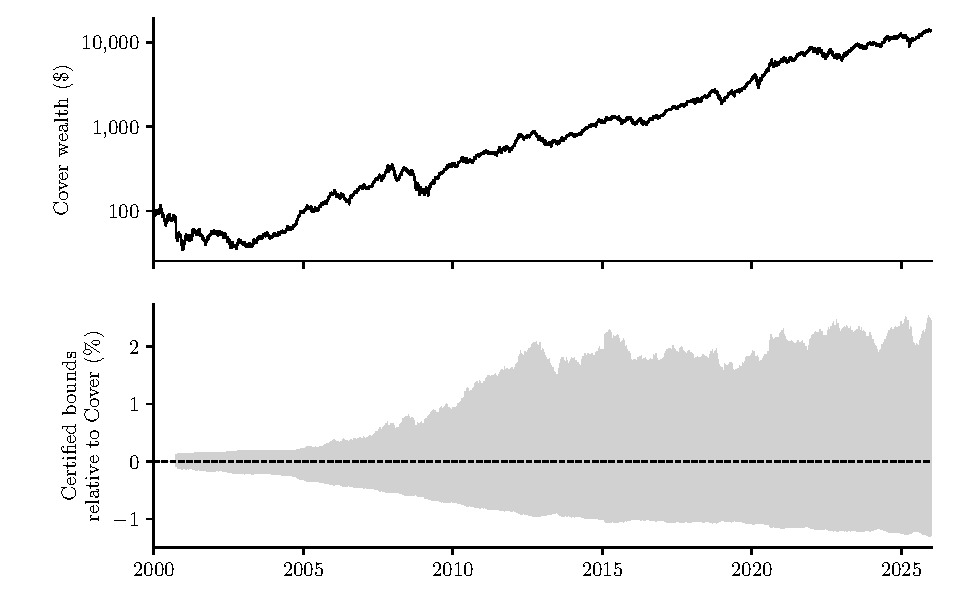
\includegraphics[width=0.83\linewidth]{aapl_msft_pair_series.pdf}
\caption{Cover's wealth on AAPL and MSFT, 2000--2025, with bounds
computed using the pair series of Lemma~\ref{lem:pair-series}. The upper
panel shows the value of an initial \$100 on a log scale, while the lower
panel takes the directly integrated Cover wealth $Z_t$ as its reference
at zero. The shaded band therefore runs from $100(L_t/Z_t-1)$ to
$100(U_t/Z_t-1)$ percent, where $L_t,U_t$ are the certified wealth
endpoints.}
\label{fig:aapl}
\end{figure}

Figure~\ref{fig:fifty} gives the corresponding results for 50 stocks,
using daily adjusted closing prices from Yahoo Finance \citep{yahooprices,yfinance}.
Within each of ten industry groups, we took the first five candidate
tickers with a positive adjusted close on every SPY trading date
from 31 December 1999 to 31 December 2025.
This choice allowed us to hold the universe fixed for all 6,539 returns
without imputing missing prices, although it favors surviving stocks.

On this panel, an initial \$100 invested in Cover grew to an estimated
\$1,771.00. The pooled estimate from eight independently scrambled Sobol
nets (Appendix~\ref{app:equity-protocol}) lay inside the band on all 6,539 closes,
and the largest deviation of a single-net estimate from the pooled
reference was $1.52\times10^{-7}$ log units. At the final close the band
extended from 0.0086\% below the estimate to 0.0497\% above it, and
its greatest width over the full period was 0.062 percentage points.
Computing the evidence interval at every close took 55 seconds.

\begin{figure}[!htbp]
\centering
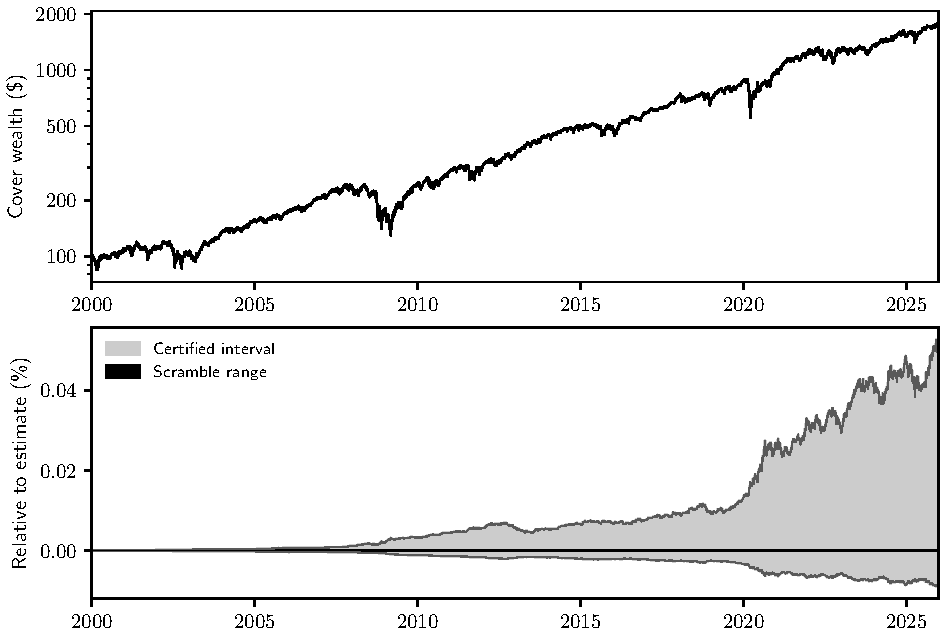
\includegraphics[width=0.83\linewidth]{fig2_50stock.pdf}
\caption{Cover's wealth on the 50-stock panel, 2000--2025. The upper
panel shows the estimated value of an initial \$100 on a log scale.
In the lower panel, both the certified band (gray) and the range of eight
scrambled Sobol estimates (black) are expressed as percentages relative
to the pooled estimate. The returns and prior alone determine the
certified band.}
\label{fig:fifty}
\end{figure}

The terminal band on the 50 stocks is about 64 times narrower than on
the pair. To see how the dimension enters this comparison, recall that
under the uniform prior the variance of a centered daily payoff is
$\|a_s\|^2/[d(d+1)]$. If the cross-sectional mean
$d^{-1}\|a_s\|^2$ stays bounded, this variance falls as $O(1/d)$.
The smaller Jensen contribution on the larger panel
(Table~\ref{tab:curvature-slack}) is consistent with this concentration
of payoffs around their equal-weight value.

\FloatBarrier
\section{A certified benchmark for online portfolio selection}\label{sec:bench}

On six standard portfolio benchmarks, we use the certified interval both
to measure how closely competing strategies tracked Cover and to check
the wealth attributed to Cover in earlier studies. The six markets come
from the OLPS toolbox \citep{li2016olps}, with their dimensions and dates
given in Table~\ref{tab:bench-accuracy}. We use the published price relatives
as supplied, including the five rows with an entry outside $[0.5,2]$.
Since all entries are positive, we take
$S=\emptyset$ by default. For the scaling experiment we also use FinOL
NYSE(N) and FinOL SP500 \citep{finol}.

Under the uniform prior, we compare Cover with the first-order
rule~\eqref{eq:first-order}, sampled UP, Soft-Bayes \citep{orseau2017}
and VB-FTRL \citep{jezequel2026}. For sampled UP, \citet{blumkalai1999}
assign equal initial capital to $M$ portfolios drawn from the prior, so
their first allocation is the sample mean. Our variant starts at 1/N,
as do the other strategies, and then weights each sampled portfolio by
the wealth it would have earned over all preceding days.
We repeat the experiment with five independent draws of the entire sample
for each $M\in\{10^2,10^3,10^4,10^5\}$. For Soft-Bayes we use the
horizon-dependent learning rate $\eta=q/(1+q)$ with
$q=\sqrt{\log(d)/(dT)}$, and for VB-FTRL we use the published
finite-iteration schedule with $(\lambda,\mu)=(560,2)$.

All strategies trade without costs. We also compare
Cover with 1/N itself, whose normalized log wealth is zero, so that the
evidence interval directly encloses the gap. For an independent estimate
of Cover's wealth we use the same Sobol quadrature as on the 50-stock
panel (Appendix~\ref{app:equity-protocol}).

\subsection{Accuracy of the certificate}
To compare the size of the certificate with the error it bounds, let
$B=\max_{t\le T}\max\{-\Delta_t^-,\Delta_t^+\}$ denote the certified
peak error and $E=\max_{t\le T}|\log\widehat Z_t-\log V_t|$ the peak
error measured against the numerical reference $\widehat Z_t$. On the
four shorter datasets, the uniform-prior evidence interval was at most
$4.4\times10^{-5}$ wide, and we could certify that the first-order rule
was within $10^{-4}$ of Cover's log wealth at every close. On NYSE(O)
and NYSE(N), the peak widths reached $0.00605$ and $0.00782$,
respectively, with $10^{-2}$ the smallest tolerance we could verify on
our grid. Across the two priors, $\alpha=1$ and $\alpha=1/2$, the
evidence interval contained the pooled reference at all 32{,}334
dataset--prior closes.

\begin{table}[tbp]
\centering
\caption{Dataset characteristics and uniform-prior accuracy. Final and maximum
evidence widths and the first-order bound $B$ are in units of $10^{-4}$ log
wealth, rounded up. The column $\varepsilon$ is the smallest of
$10^{-5},10^{-4},10^{-3},10^{-2},10^{-1}$ that bounds the first-order error
at every close, in unscaled log units. The last column times all daily
evidence evaluations for that market.}
\label{tab:bench-accuracy}
\small\setlength{\tabcolsep}{3.1pt}
\begin{tabular}{@{}lrrlrrrrrrr@{}}
\toprule
 & & & & & \multicolumn{2}{c}{Width} & \multicolumn{3}{c}{First-order Cover} & \\
\cmidrule(lr){6-7}\cmidrule(lr){8-10}
Market & $d$ & $T$ & Period & $\min_s m_s$ & Final & Max. &
$B$ & $B/E$ & $\varepsilon$ & Time (s)\\
\midrule
NYSE(O) & 36 & 5,651 & 1962--1984 & .7576 & 40.4 & 60.5 & 44.9 & 3.58 & $10^{-2}$ & 26.6\\
NYSE(N) & 23 & 6,431 & 1985--2010 & .4493 & 77.2 & 78.2 & 53.5 & 1.58 & $10^{-2}$ & 14.5\\
DJIA    & 30 &   507 & 2001--2003 & .4121 & .0440 & .0440 & .142 & 1.12 & $10^{-4}$ & 1.7\\
SP500   & 25 & 1,276 & 1998--2003 & .7202 & .426 & .434 & .877 & 1.18 & $10^{-4}$ & 3.2\\
MSCI    & 24 & 1,043 & 2006--2010 & .8247 & .0273 & .0273 & .185 & 1.09 & $10^{-4}$ & 2.5\\
TSE     & 88 & 1,259 & 1994--1998 & .3710 & .0600 & .0602 & .168 & 1.28 & $10^{-4}$ & 27.6\\
\bottomrule
\end{tabular}
\end{table}

Across the 144 allocation histories in Table~\ref{tab:bench-gaps}, the
median $B/E$ was $1.003$, so the certified bound was typically close to
the measured peak error. The largest ratio, $30.05$, occurred for one
$M=10^5$ sample on NYSE(N), where the measured peak error of
$2.31\times10^{-4}$ was substantially smaller than the uncertainty in
Cover's log wealth.

\subsection{Certified gaps}\label{sec:bench-gaps}
On DJIA, SP500, MSCI and TSE, the terminal certificate placed the
first-order rule within $6.6\times10^{-5}$ of Cover in log wealth and
determined the sign of the gap on each market
(Table~\ref{tab:bench-gaps}). The daily intervals also show how long a
difference persisted. On DJIA, for example, the first-order rule was
certified behind Cover on 475 of the 507 closes and ahead on 17, leaving
only 15 closes undecided.

For sampled UP, even the best of the five samples of $10^5$ portfolios
had a measured peak error between 3.2 and 14 times the first-order
error across these four markets. On each market at least one sample
finished certified ahead of Cover and one finished certified behind.
Increasing the sample size nevertheless reduced the spread of the
terminal gaps, with the largest absolute terminal endpoint on DJIA
falling by a factor of about 35 from $M=10^2$ to $M=10^5$.

\begin{table}[tbp]
\centering
\caption{Certified terminal gap $\Delta_T=\log Z_T-\log V_T$ in units of
$10^{-4}$ log wealth, rounded outward. Positive values mean Cover finished
ahead. For sampled UP we give the smallest interval containing the five
certified intervals, one per independent draw. A dagger means that one draw
finished certified ahead of Cover and another behind.}
\label{tab:bench-gaps}
\begingroup
\setlength{\tabcolsep}{2.5pt}\footnotesize
\resizebox{\linewidth}{!}{%
\begin{tabular}{@{}lcccccc@{}}
\toprule
Strategy & NYSE(O) & NYSE(N) & DJIA & SP500 & MSCI & TSE\\
\midrule
First-order Cover & $[-16.22,24.17]$ & $[-23.68,53.48]$ & $[0.07,0.13]$ & $[-0.66,-0.22]$ & $[-0.16,-0.13]$ & $[0.10,0.17]$\\
Sampled UP, $10^2$ & $[-318.97,282.84]^\dagger$ & $[-635.14,308.94]^\dagger$ & $[-26.25,74.43]^\dagger$ & $[-73.86,162.27]^\dagger$ & $[-171.67,89.48]^\dagger$ & $[-153.06,81.01]^\dagger$\\
\phantom{Sampled UP, }$10^3$ & $[-113.65,117.66]^\dagger$ & $[-190.94,225.02]^\dagger$ & $[2.49,35.44]$ & $[-11.44,22.73]^\dagger$ & $[-25.52,15.23]^\dagger$ & $[-67.42,18.21]^\dagger$\\
\phantom{Sampled UP, }$10^4$ & $[-31.99,74.48]$ & $[-33.46,127.00]$ & $[-2.96,6.54]^\dagger$ & $[-9.44,10.34]^\dagger$ & $[-8.03,10.51]^\dagger$ & $[-1.17,15.43]^\dagger$\\
\phantom{Sampled UP, }$10^5$ & $[-14.23,43.96]$ & $[-21.07,77.64]$ & $[-1.40,2.15]^\dagger$ & $[-6.57,3.13]^\dagger$ & $[-3.18,5.81]^\dagger$ & $[-0.27,2.47]^\dagger$\\
Soft-Bayes & $[-11.68,28.71]$ & $[-157.62,-80.46]$ & $[-11.62,-11.56]$ & $[-53.89,-53.46]$ & $[-5.22,-5.18]$ & $[-0.97,-0.90]$\\
VB-FTRL & $[-10.96,29.43]$ & $[-173.78,-96.62]$ & $[-21.38,-21.33]$ & $[-72.32,-71.88]$ & $[-7.16,-7.12]$ & $[-2.29,-2.22]$\\
1/N & $[-10.95,29.44]$ & $[-174.05,-96.89]$ & $[-21.42,-21.37]$ & $[-72.45,-72.01]$ & $[-7.17,-7.14]$ & $[-2.30,-2.23]$\\
\bottomrule
\end{tabular}}
\endgroup
\end{table}

On NYSE(O) and NYSE(N), the terminal evidence intervals were about 40
and 77 units of $10^{-4}$ wide, respectively, and both first-order gap
intervals contained zero. At $M=10^5$ the certificate left three of the
five draws undecided on each market and placed the other two behind
Cover. On these longer paths, however, all five draws gave a smaller
measured peak error than the first-order rule. On NYSE(O) and NYSE(N) the first-order errors were $1.25\times10^{-3}$
and $3.38\times10^{-3}$,
respectively, compared with ranges of $0.48$--$1.21\times10^{-3}$ and
$0.23$--$1.35\times10^{-3}$ for sampled UP. The expansion behind~\eqref{eq:first-order}
assumes small returns at fixed horizon, which limits what it can
explain about these longer paths.

On every market the terminal log wealth of VB-FTRL was within
$3\times10^{-5}$ of 1/N, while that of Soft-Bayes was within
$2\times10^{-3}$. We could certify that all three finished ahead of Cover
on NYSE(N), DJIA, SP500, MSCI and TSE, whereas the interval on NYSE(O)
left all three comparisons undecided. Figure~\ref{fig:bench-wealth}
shows how their wealth evolved on NYSE(N) and DJIA.

\begin{figure}[tbp]
\centering
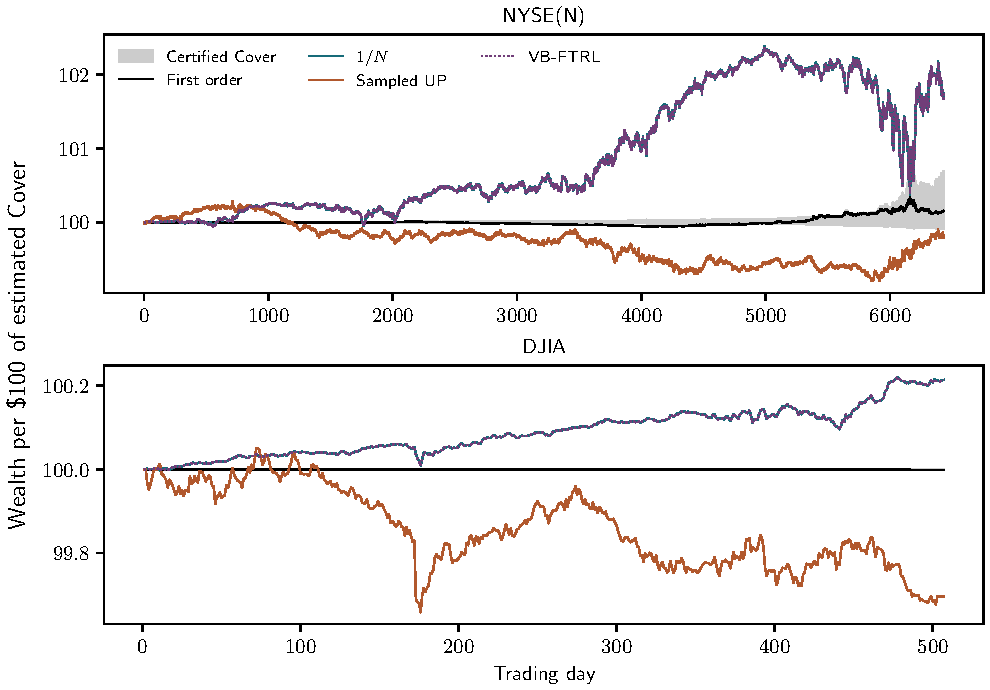
\includegraphics[width=.87\linewidth]{bench_wealth.pdf}
\caption{Strategy wealth per \$100 of estimated Cover wealth on NYSE(N)
and DJIA. Gray shows the certified Cover interval on that scale.
Sampled UP uses $M=1{,}000$ and the first of the five draws.
The VB-FTRL and 1/N curves overlap at this scale.}
\label{fig:bench-wealth}
\end{figure}

\subsection{Audit of published universal-portfolio wealths}\label{sec:audit}
Several papers report universal-portfolio wealth on these markets to two
decimal places. To determine whether the published values agree with
continuous uniform-prior Cover to that precision, we compare them with
our certified intervals and with our replay of the OLPS toolbox
(Table~\ref{tab:bench-audit}). Only on DJIA could rounding Cover's
terminal wealth to cents give the published figure. On the other five
markets the published figures differ from the interval midpoint by
approximately 0.3\% to 1.6\%, with the two SP500 values, \$1.62 and
\$1.65, lying on opposite sides of the certified interval.

\citet{hindawi2020} set transaction costs to zero and specify $m=100$
and $S=500$ for their random-walk sampler, while
\citet{mathematics2022} use implementations provided by Li and
coauthors and report the zero-cost baseline in Table~A2. For our comparison
we ran the original OLPS toolbox with zero transaction costs.

\begin{table}[tbp]
\centering
\caption{Terminal wealth per initial dollar. The interval encloses
uniform-prior Cover wealth. The toolbox column gives our MATLAB replay,
and the published column gives the UP wealth reported by each source. The toolbox
gap is $\Delta_T$ in $10^{-4}$ log units, rounded outward. The sample range
gives the five terminal wealths' minimum and maximum, rounded outward.
Published values come from \citet[Table~1(a)]{li2012olmar} for NYSE(O),
NYSE(N), DJIA and TSE and from \citet[Table~3]{hindawi2020} and
\citet[Table~A2]{mathematics2022} for all six markets. The two SP500 entries
are in the latter sources' order.}
\label{tab:bench-audit}
\small\setlength{\tabcolsep}{4pt}
\begin{tabular}{@{}lccccr@{}}
\toprule
 & Certified Cover & Toolbox & Toolbox gap & Sampled UP & Published\\
Market & (\$) & (\$) & ($10^{-4}$ log) & $M=10^5$ (\$) & (\$)\\
\midrule
NYSE(O) & $[27.045635,27.155072]$ & 27.065128 & $[-7.21,33.18]$ & 27.0359--27.0842 & 26.68\\
NYSE(N) & $[31.007309,31.247456]$ & 31.557981 & $[-176.04,-98.88]$ & 31.0057--31.0728 & 31.49\\
DJIA & $[0.810987,0.810991]$ & 0.810639 & $[4.29,4.34]$ & 0.8108--0.8112 & 0.81\\
SP500 & $[1.636812,1.636883]$ & 1.646159 & $[-56.94,-56.50]$ & 1.6363--1.6379 & 1.62, 1.65\\
MSCI & $[0.926172,0.926175]$ & 0.924282 & $[20.42,20.46]$ & 0.9256--0.9265 & 0.92\\
TSE & $[1.594859,1.594870]$ & 1.587951 & $[43.40,43.47]$ & 1.5944--1.5950 & 1.60\\
\bottomrule
\end{tabular}
\end{table}

Each day the toolbox averages the endpoints of short random walks from
equal weights, with a floor on each portfolio weight. The resulting terminal
wealth lay inside the certified interval on NYSE(O). On the other five
markets it lay outside, differing from the interval midpoint by between
0.04\% and 1.4\% in absolute value. On MSCI and SP500 this difference
persists after rounding to cents, with the MATLAB replay giving
\$0.92 and \$1.65, respectively, and Cover giving \$0.93 and
\$1.64. On NYSE(N) the difference changes the ranking, since the
toolbox finished 0.02\% ahead of 1/N while Cover finished between
0.96\% and 1.73\% behind.

For sampled UP with $M=10^5$, every one of the five draws on each of
the six markets finished either inside the certified interval or within
0.062\% of the nearer endpoint. When the interval is wide, a sampled
wealth that falls inside it can still differ appreciably from Cover's
wealth.

\subsection{Cost and scaling}\label{sec:cost}
To examine how the cost depends on dimension and horizon, we certified
every close on nested subsets of FinOL NYSE(N)
(Table~\ref{tab:bench-cost}). At fixed horizon the fitted exponents for
dimension ranged from 1.83 to 1.84, whereas at fixed dimension the
exponents for the horizon ranged from 1.01 to 1.03
(Figure~\ref{fig:bench-scale}). On the full 403-stock panel the
pair-series degree reached 172, with a median runtime of 48 minutes
12 seconds and median peak memory of 465~MiB. On the six classic
markets, a single evidence calculation took 1.7--28 seconds and served
all the portfolios on that market. For comparison, generating the
allocations alone took 1.1--346 seconds for VB-FTRL and at most
0.042 seconds for the first-order rule.

\begin{table}[tbp]
\centering
\caption{Cost of the pair-series evidence interval at every close, on the
first $d$ assets and first $T$ days of FinOL NYSE(N). Times are medians of
three single-threaded runs on an Apple M1 Pro, including initialization,
updates and endpoint evaluation. Final widths are in log units, rounded up,
and memory is median peak resident set size. On FinOL SP500 ($d=339$, $T=1{,}277$)
the corresponding figures were 374 seconds, 359~MiB and a width below
$6.1\times10^{-7}$.}
\label{tab:bench-cost}
\small
\begin{tabular}{@{}rrrrrrr@{}}
\toprule
 & \multicolumn{4}{c}{Wall time (s)} & \multicolumn{2}{c}{$T=6{,}430$}\\
\cmidrule(lr){2-5}\cmidrule(l){6-7}
$d$ & $T=1{,}000$ & $2{,}000$ & $4{,}000$ & $6{,}430$ & Peak MiB & Final width\\
\midrule
25 & 2.63 & 5.27 & 10.5 & 17.2 & 127 & $4.2\times10^{-3}$\\
50 & 7.95 & 16.1 & 32.5 & 52.8 & 131 & $1.4\times10^{-3}$\\
100 & 27.3 & 55.3 & 112 & 181 & 158 & $6.3\times10^{-4}$\\
200 & 104 & 208 & 421 & 679 & 238 & $3.5\times10^{-3}$\\
403 & 424 & 853 & 1,768 & 2,892 & 465 & $2.833$\\
\bottomrule
\end{tabular}
\end{table}

\begin{figure}[tbp]
\centering
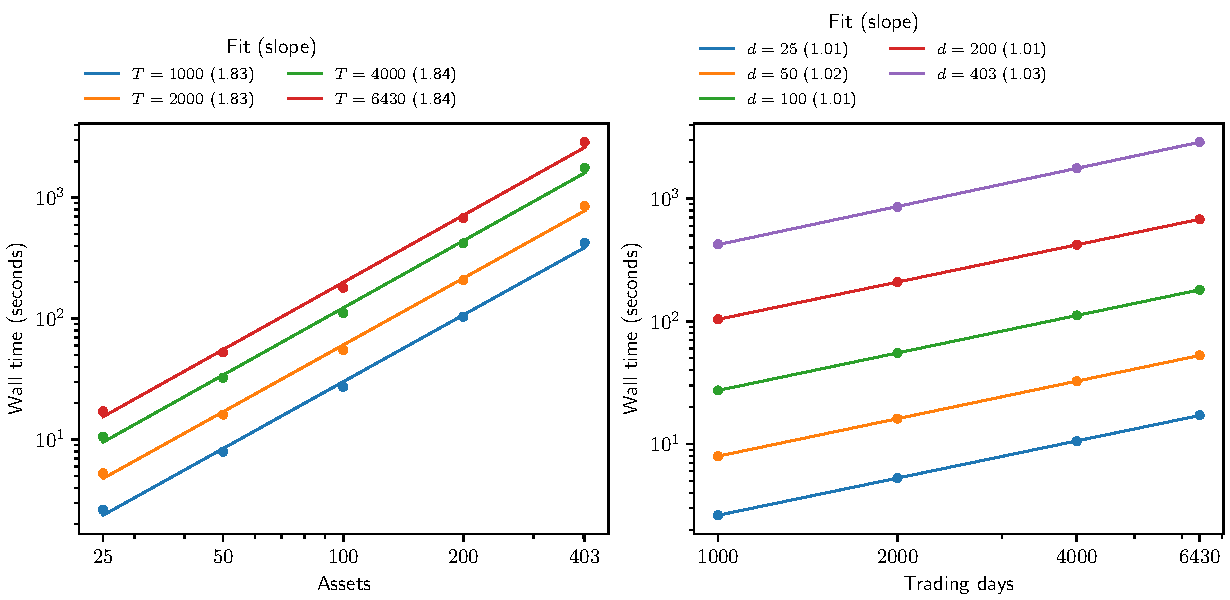
\includegraphics[width=\linewidth]{bench_scaling.pdf}
\caption{Evidence runtime on FinOL NYSE(N) as dimension varies at fixed
horizon (left) and horizon varies at fixed dimension (right). Points are
median times. Lines are log--log least-squares fits with slopes given
in the legends.}
\label{fig:bench-scale}
\end{figure}

On 2 December 1988 CIA's price relative was $0.07292$, giving
$m_s=0.07282$, the smallest normalized price relative on the
403-stock panel. To examine the width on this panel, we first omitted the bound
$|I(J)|\le I(C)$ of Lemma~\ref{lem:streaming-moments}. The Taylor
enclosure of $I(J)$ then dominated the width because its remainder
contains the factor $\rho_3(L)$, which grows exponentially in $L$.
By day 4,000 the width exceeded $10^7$ log units, reaching
$4.1643\times10^7$ at the final close, rounded up. Applying the bound
used throughout the paper reduced the final width to $2.832558$ log
units, rounded up, with all rows still in the expansion.

We next kept the one to five rows with the smallest $m_s$ exact.
The intersection of the resulting intervals was $[-2.824625,0.007878]$,
rounded outward, so the additional reduction in width was at most
$5.55\times10^{-5}$ log units. On five of the six classic markets,
keeping the row with the smallest $m_s$ exact gave a wider terminal
interval than $S=\varnothing$. The exception was NYSE(N), where keeping
that row exact reduced the width from $0.007715$ to $0.007566$ log
units, both rounded up.

For $d=25$ and $T=1{,}000$, the Taylor checkpoint took 0.92 seconds
and the pair series took 2.63 seconds, although their widths differed
by less than 0.6\%. The additional pair moments made a larger
difference on AAPL--MSFT, where they reduced the terminal band from
about 5.97 to 3.74 percentage points (Section~\ref{sec:examples}).

\subsection{Certified regret}
To enclose hindsight regret, we maximize the log wealth
$f(w)=\sum_{s\le T}\log(w^\top x_s)$ on each market and use the
Frank--Wolfe gap $\max_i\nabla_i f(w)-w^\top\nabla f(w)$ to bound the
difference between the optimum and the computed value $f(w)$.
The computed gaps were below $5\times10^{-7}$ in directed arithmetic.
Subtracting Cover's certified log wealth from the resulting intervals
for the optimum gives regret intervals of $[2.222,2.227]$ on NYSE(O),
$[1.348,1.356]$ on NYSE(N), $[0.424,0.425]$ on DJIA, $[0.910,0.911]$
on SP500, $[0.485,0.486]$ on MSCI and $[1.447,1.448]$ on TSE, all in
log units and rounded outward. The worst-case bound
$\log\binom{T+d-1}{d-1}$ in Corollary~\ref{cor:prefix-regret} was thus
94 to 260 times as large as Cover's realized regret on these markets.
Since first-order regret differs from Cover's by $\Delta_T$, their
regrets were within $10^{-4}$ of one another on the four shorter
datasets.

\FloatBarrier
\section{Is Cover's lead over equal weighting real?}
\label{sec:test}

Even when 1/N is growth-optimal, Cover can accumulate more wealth
over a particular period. We therefore ask how large this lead must be
to provide evidence against conditional growth optimality. Since we
observe the wealth ratio at every close, the test must remain valid
when the investor chooses when to stop.

\subsection{A certified anytime-valid test}
Let $r_{s,i}=x_{s,i}/\bar x_s$, and let $\mathcal F_s$ contain the
information available at close $s$. We test the hypothesis
\begin{equation}\label{eq:h0}
 H_0:\qquad \E[r_{s,i}\mid\mathcal F_{s-1}]=1
 \quad\text{for each asset $i$ and day $s$.}
\end{equation}
To see why this is the relevant hypothesis, consider the portfolio
$u=\one/d$, whose payoff in units of 1/N is one. The directional
derivative of conditional expected log growth from $u$ towards asset $i$
is then $\E[r_{s,i}-1\mid\mathcal F_{s-1}]$. By concavity, $u$ is
optimal exactly when these derivatives are all nonpositive, and since
$\sum_i r_{s,i}=d$, their sum is zero. At an optimum every derivative
must therefore vanish, giving \eqref{eq:h0} as the condition for 1/N to be the
conditionally growth-optimal, or num\'eraire, portfolio. Taking 1/N as
the index connects our discrete-time test to the efficient-index
question studied by \citet{vovk2011efficient} and
\citet{vovk2016probabilityfree}.

\begin{proposition}[Anytime-valid test]\label{prop:ville}
Under \eqref{eq:h0}, for any prior fixed in advance and any
$\delta\in(0,1)$, a lower endpoint $z_t^-$ of the evidence interval
computed through close $t$ satisfies
\[
  \mathbb P\!\left(\exists\,t\ge1:\ z_t^-\ge\log(1/\delta)\right)
  \le\delta .
\]
\end{proposition}
\begin{proof}
Under the null hypothesis, the next payoff of each fixed portfolio $w$ has
conditional mean one, so its wealth $\prod_{s\le t}w^\top r_s$ is a
nonnegative martingale starting at one. By conditional Tonelli, its
prior average $\bar Z_t$ is also a nonnegative martingale starting at
one. Ville's inequality bounds the probability that this mixture ever
reaches $1/\delta$ by $\delta$, and the result follows since
$e^{z_t^-}\le\bar Z_t$ at each close.
\end{proof}

We reject on the first close at which the lower e-value
$e^{z_t^-}$ reaches $1/\delta$. Although a wider enclosure can delay
rejection, the false-rejection bound holds even when the investor
chooses when to stop. Since Cover averages the wealth of fixed
rebalanced portfolios, the test can have little power against
predictable changes that require switching between portfolios.

For these experiments we fixed the uniform prior, set $\delta=0.05$
(threshold 20) and monitored the lower e-value at every close. For the
primary market we used Yahoo Finance adjusted closes
\citep{yahooprices,yfinance} for the nine original Select
Sector SPDRs from January 1999 to December 2025, with the six OLPS datasets
and the 50-stock panel as secondary markets. All eight market histories
had been examined previously. To account for the eight comparisons, we also applied e-BH at
level $0.05$ to the \emph{terminal} lower e-values \citep{wang2022false}.

\subsection{Eight markets}
The sector panel reached its largest lower e-value of 1.0017 on
1 July 2008 before finishing below one, while the largest secondary
peak was 1.0044 on SP500 (Table~\ref{tab:evalues}). On all eight
markets even the upper e-value stayed below 1.010 at every close, so
the exact mixture never reached the threshold of 20
(Figure~\ref{fig:evalues}). Neither the certified test on the individual histories nor e-BH
applied to the eight terminal values gave a rejection.

The interval nevertheless determined the sign of the terminal wealth difference on seven markets,
in each case agreeing with the prediction of \eqref{eq:second-order}.
The remaining market, NYSE(O), was the only one with $\mathrm{VR}_T>1$,
and its terminal e-value interval straddled one.

\begin{table}[!htbp]
\centering\small
\caption{Cover wealth in units of 1/N on the eight markets. The terminal
e-value intervals are rounded outward. The peak is the largest certified
lower e-value over trading closes, rounded down. The final column compares
the sign of \eqref{eq:second-order} with the certified sign of
$\log\bar Z_T$. An interval containing one leaves the sign undecided.}
\label{tab:evalues}
\begin{tabular}{lrrcccc}
\toprule
Market & $d$ & $T$ & Terminal e-value & Peak lower & $\mathrm{VR}_T$ &
Prediction\\
\midrule
Sector panel & 9 & 6,791 & $[0.9782,0.9785]$ & 1.0017 & 0.167 & agrees\\
NYSE(O) & 36 & 5,651 & $[0.9989,1.0030]$ & 1.0038 & 1.023 & undecided\\
NYSE(N) & 23 & 6,431 & $[0.9827,0.9904]$ & 1.0005 & 0.700 & agrees\\
DJIA & 30 & 507 & $[0.9978,0.9979]$ & 1.0000 & 0.355 & agrees\\
SP500 & 25 & 1,276 & $[0.9927,0.9929]$ & 1.0044 & 0.368 & agrees\\
MSCI & 24 & 1,043 & $[0.9992,0.9993]$ & 1.0000 & 0.781 & agrees\\
TSE & 88 & 1,259 & $[0.9997,0.9998]$ & 1.0006 & 0.934 & agrees\\
50-stock panel & 50 & 6,539 & $[0.9954,0.9961]$ & 1.0020 & 0.716 & agrees\\
\bottomrule
\end{tabular}
\end{table}

\begin{figure}[!htbp]
\centering
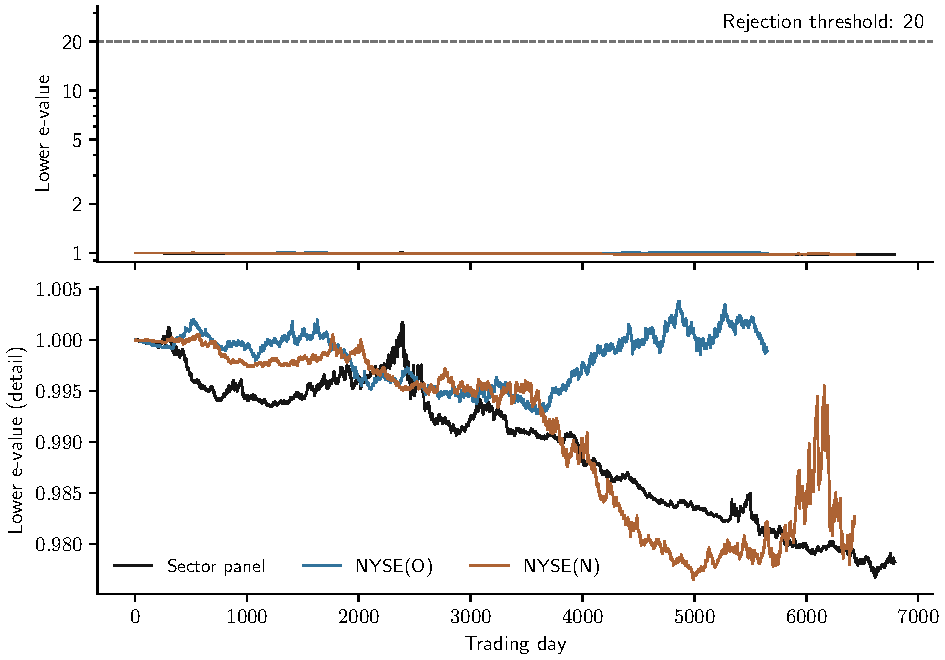
\includegraphics[width=0.84\linewidth]{evalue_1overN.pdf}
\caption{Certified lower e-values on the sector panel, NYSE(O) and
NYSE(N), by elapsed trading day. The upper panel shows the rejection
threshold of 20 on a log scale. The lower panel shows the same paths
near one.}
\label{fig:evalues}
\end{figure}

\subsection{Validation}
To check the stopping rule against direct integration, we used the
technology and utilities sector ETFs (XLK and XLU). The evidence
interval enclosed the Bernstein integral at all 6,791 closes, and an
independent Gauss--Legendre calculation agreed with the integral
to within $1.9\times10^{-14}$ log units. Neither the integral nor the
certified lower endpoint reached 20 on the observed returns. We
therefore repeated the comparison on the same pair with an 80\% annual
log-growth gap planted as described below, in which case both first
crossed on day 3,522.

To generate histories satisfying \eqref{eq:h0} exactly, we independently
permuted the asset labels in each observed row. This preserves each
day's cross-sectional spread while giving every coordinate conditional
mean one given the past and that day's row. We observed zero rejections
in 1,000 sector replays and zero in 200 DJIA replays, giving upper
endpoints of 0.37\% and 1.83\%, respectively, for the two-sided 95\%
Clopper--Pearson intervals \citep{clopper1934}.

\subsection{Why the evidence builds slowly}
To examine how a persistent advantage accumulates in the mixture,
we added a fixed daily drift to each asset's log return on each of 200
independently relabeled sector histories and renormalized by the new
1/N payoff. We spaced the annualized drifts equally from $-g/2$ to
$g/2$, giving a best-to-worst annual log-growth gap of
$g\in\{5,10,20,40,80\}\%$. The e-value stayed below 20 throughout the 6,791 days of all 200
replays at every gap, and a separate upper bound ruled out a crossing
of 20 by the exact mixture. The same held at 5\% and 10\% when we extended the
histories to 25,000 days by independently relabeling each pass. On the first replay at the 80\% gap the
winning sector grew to 10,533 times the wealth of 1/N, whereas Cover's
terminal wealth in the same units lay in $[8.11,8.32]$.

We can quantify the cost of averaging when the best constant-rebalanced
portfolio consists of a single asset $j$. Assume $x_{s,j}>0$ at every
close and write $\Gamma=t^{-1}\log
\{S_t(e_j)/V_t^{1/N}\}$ and $c_i=t^{-1}\sum_{s\le t}
(1-x_{s,i}/x_{s,j})$ for $i\ne j$. If each slope is strictly
positive, moving weight $u_i$ from the vertex towards asset $i$ incurs
a first-order log-wealth loss of $tc_i u_i$. When the integral is
concentrated near that vertex, integrating the exponential of the
negative linear loss over its tangent cone gives the uniform-prior
approximation
\[
 \log\bar Z_t \approx t\Gamma+\log\bigl((d-1)!\bigr)
                         -\sum_{i\ne j}\log(tc_i).
\]
Here the factorial is the density of the uniform prior in these
coordinates. On the first 80\% replay the directional derivatives
certified a strict vertex optimum, so we used $\Gamma$ as a common
scale for the $c_i$ to estimate the size of the penalty. At the
observed horizon this gives 2.059, compared with the certified log
interval $[2.094,2.118]$. Extrapolating along the increasing branch of
the common-slope approximation on this one path gives a crossing of 20
after roughly 9,400 trading days, or 37 years. The penalty depends on the number of directions in which the
prior assigns capital away from the winner.

\subsection{Number of assets}
To study the effect of the number of assets, we repeated the
comparison with 1/N on all 1,225 pairs from the 50-stock panel, 200 random
subsets at each of four intermediate sizes, and the full panel.
Of the 2,026 subsets, Cover finished certified ahead of 1/N on 352 and
behind on 1,601, leaving 73 comparisons undecided. An independent upper
bound on the exact mixture stayed below 20 at every close of every
subset. Thus even where we could establish a realized advantage for
Cover, its magnitude provided little evidence against conditional
growth optimality.

\begin{table}[!htbp]
\centering\small\setlength{\tabcolsep}{3.5pt}
\caption{Terminal Cover wealth relative to 1/N by subset size.
Ahead and behind refer to the certified sign of
$\Delta_T=\log(Z_T/V_T^{1/N})$. The median and quartiles use interval
midpoints in units of $10^{-4}$ log wealth. The two stratified columns
give the percentage certified ahead conditional on the presence of a
top-five stock. The last column gives the largest Arb lower e-value
at the screened candidate closes for the subsets and across all closes
for the full panel, rounded down to hundredths.}
\label{tab:subsets}
\begin{tabular}{rr rrr r rr r}
\toprule
 & & \multicolumn{3}{c}{Terminal verdict (\%)} & $\Delta_T/10^{-4}$ &
 \multicolumn{2}{c}{Ahead (\%)} & Peak\\
\cmidrule(lr){3-5}\cmidrule(lr){7-8}
$d$ & Subsets & Ahead & Behind & Open & Median [quartiles] &
Top five & None & lower\\
\midrule
2 & 1,225 & 15.5 & 81.8 & 2.7 & $-743\,[-1154,-280]$ & 43.4 & 8.9 & 3.11\\
3 & 200 & 14.5 & 80.0 & 5.5 & $-631\,[-1036,-237]$ & 34.5 & 6.3 & 1.76\\
5 & 200 & 12.5 & 83.0 & 4.5 & $-521\,[-798,-260]$ & 31.6 & 0.0 & 1.42\\
10 & 200 & 20.0 & 79.5 & 0.5 & $-290\,[-389,-157]$ & 27.4 & 0.0 & 1.09\\
20 & 200 & 34.0 & 56.5 & 9.5 & $-143\,[-201,75]$ & 36.4 & 0.0 & 1.02\\
50 & 1 & 0.0 & 100.0 & 0.0 & $-42$ & 0.0 & --- & 1.00\\
\bottomrule
\end{tabular}
\end{table}

\begin{figure}[!htbp]
\centering
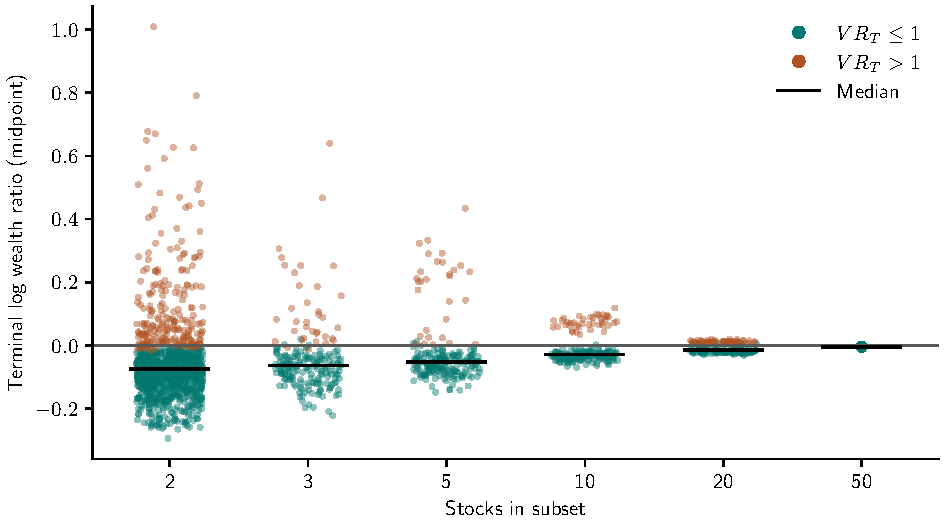
\includegraphics[width=0.86\linewidth]{subsets_1overN.pdf}
\caption{Terminal log wealth of Cover relative to 1/N by number of
stocks. Each point is the midpoint of a subset's certified interval.
Color distinguishes variance ratios above and below one. The horizontal
line marks equality of terminal wealth.}
\label{fig:subsets}
\end{figure}

Among the pairs, the largest and smallest directly integrated wealth
ratios were 2.54 on Apple--Citigroup and 0.75 on Bank of
America--Newmont, with Apple--Citigroup also attaining the largest
checked lower e-value of approximately 3.11. The five stocks with the highest buy-and-hold returns over the
full period were AAPL, CAT, DE, EOG and NUE. Among pairs containing at
least one of these stocks, Cover finished certified ahead on 43.4\%,
compared with 8.9\% of the remaining pairs.
At $d=5,10,20$ all 133 certified wins contained a top-five stock
(Table~\ref{tab:subsets}).

As the number of assets increased, the median log ratio moved towards
zero (Figure~\ref{fig:subsets}), as suggested by the denominator in
\eqref{eq:second-order}. The predicted sign agreed with 1,937 of the
1,953 signs determined by the certificate, and all 1,225 independent
terminal pair integrals lay inside their enclosures. Since the subsets
share dates and constituents, the top-five classification uses
full-period returns and the complete-history requirement favors
survivors, these comparisons describe the dispersion of outcomes on
this particular panel. Convergence of diversified portfolios to the
num\'eraire requires separate assumptions
\citep{platen2012approximating}.

\FloatBarrier
\section{Discussion}

Once we have enclosed Cover's wealth on a return history, we can use the
same interval to compare any strategy with positive payoffs on that history.
The precision of the comparison depends on the returns. On the four shorter
benchmarks the certificate resolved terminal differences of order $10^{-5}$
in log wealth, whereas on the two longer NYSE datasets its peak log width
reached 0.0061 and 0.0079, respectively, leaving the sign of the first-order
gap undecided at the last close.

The width decomposition helps identify which part of the calculation would
benefit from a sharper bound. On the 50-stock panel, enclosing the tilted
moments accounted for about 93\% of the implemented width, so improving
these moment bounds would directly improve the precision of the benchmark.
On the 403-stock panel, the inequality $|I(J)|\le I(C)$ controlled the cubic
term when its Taylor enclosure became too wide, although the resulting
terminal interval of about 2.83 log units was still too wide to rank close
competitors. Treating the five most extreme rows exactly narrowed the
interval by less than $0.000056$ log units (Section~\ref{sec:cost}),
while increasing the degree of the product tilt with each exact row.

Even when the score is small, the interval can be wide if the curvature
is concentrated in a single direction. Consider two stocks whose gross
returns alternate between 1.20 and 0.80 in opposite order for 12,600
sessions, with the other three stocks flat. Although the score returns to
zero after each pair of sessions, the tilted interval first became
inconclusive at tolerance 0.01 on day 56 and continued to intersect the
tolerance band thereafter. The alternating-market calculation in
Appendix~\ref{app:equity-protocol} places the first breach on day 78
by direct integration.

For the test of growth optimality, a separate question is how much wealth
the underlying mixture can accumulate against equal weighting. In the
planted sector histories even the exact uniform-prior mixture failed to
reach 20, since it assigned capital to many portfolios with little exposure
to the persistent winner. A prior concentrated near the vertices would
assign more capital to portfolios concentrated in a single stock, whereas
a switching mixture could target changes in leadership. Either modification
would define a different bet, so the choice of mixture would have to be
fixed before observing the returns used to test it.

Two features of the experiments also affect their interpretation. We
selected the Yahoo panels for complete histories, thus favoring surviving
stocks, and assumed frictionless trading in all replays. Introducing
transaction costs would change the wealth earned by the component portfolios
and hence the wealth of Cover's mixture \citep{blumkalai1999}.

\paragraph{Code and data availability.}
The code for reproducing the experiments and figures, together with
instructions for obtaining the data, is available at
\url{https://github.com/infamoussoap/CoverUniversalPortfolio}.

\begingroup
\small
\setlength{\bibsep}{1pt plus 0.4pt}
\bibliography{references}
\endgroup

\Needspace{9\baselineskip}
\appendix
\section{Evaluating the certificate}\label{sec:certificate-evaluation}

\begin{lemma}[Streaming moment enclosures]\label{lem:streaming-moments}
Suppose $S=\varnothing$ and write $\langle f\rangle=\E_\pi f(W)$ and
$L=\max_i g_i$. Given a quadratic bound $Q_A=\sum_s\eta_s y_s^2\ge D$
with $\eta_s\ge0$, define $C=\sum_s\|a_s\|_\infty y_s^2$,
$U=\sum_s\|a_s\|_\infty^2 y_s^2/(4m_s)$ and
$\sigma=\sum_s\eta_s\langle y_s^8\rangle^{1/4}$. Writing
$P_n(z)=\sum_{i=0}^n z^i/i!$ and
$\rho_n(L)=\int_0^1 (1-h)^{n-1}e^{hL}\,dh/(n-1)!$, we may take
the following moment bounds in Theorem~\ref{thm:main}.
\begin{align*}
 q^-&=\tfrac12\langle QP_3(G)\rangle,&
 q^+&=q^-+\tfrac12\rho_4(L)\langle QG^4\rangle,\\
 j^\pm&=\langle JP_2(G)\rangle\pm
 \rho_3(L)\sqrt{\langle G^2 C\rangle\langle G^4 C\rangle},&
 k^+&=\min\{e^L\langle K\rangle,\langle e^G U\rangle\}.
\end{align*}
Either term in the minimum is itself an upper bound on
$\langle e^G K\rangle$. To tighten the interval for $I(J)$, we intersect
it with $[-c^+,c^+]$, where $c^+\ge\langle e^G C\rangle$, thus replacing
$j^-$ by $\max\{j^-,-c^+\}$ and $j^+$ by $\min\{j^+,c^+\}$.
Since $C=W^\top\mathcal C W$ with
$\mathcal C=\sum_s\|a_s\|_\infty a_sa_s^\top$, we can obtain $c^+$
from the upper endpoint of $\sum_{i,k}\mathcal C_{ik}\E_\pi[e^GW_iW_k]$
using the pair series of Lemma~\ref{lem:pair-series}, whose tail bound
is independent of $\rho_n(L)$. When using the Taylor checkpoint, we
take the upper endpoint of
$\langle C P_3(G)\rangle+\rho_4(L)\langle C G^4\rangle$.
Similarly, either term in the following minimum gives a valid choice
for $b^+$, so we may take
\begin{equation}
 \min\left\{\langle(1+G)Q_A^2\rangle+
       \rho_2(L)\sqrt{\langle G^4\rangle}\,\sigma^2,\quad
       \sqrt{\langle e^{2G}\rangle}\,\sigma^2\right\}.
 \label{eq:certificate-square}
\end{equation}
\end{lemma}
\begin{proof}
By Taylor's integral remainder,
$e^G-P_{n-1}(G)=G^n\rho_n(G)$ with $0<\rho_n(G)\le\rho_n(L)$.
Since $Q\ge0$, the even remainder gives the two bounds on the quadratic
term. For the odd remainder, observe that $|y_s|\le\|a_s\|_\infty$
on the simplex and hence $|J|\le C$ pointwise. Applying Cauchy--Schwarz
to $\langle |G|^3 C\rangle$ therefore gives the square root in $j^\pm$,
while integrating the pointwise bound against the tilt gives
$|\langle e^G J\rangle|\le\langle e^G C\rangle$. The inequalities
$K\le U$ and $G\le L$ give the two upper bounds in $k^+$.

It remains to bound the square moment. By Minkowski's inequality,
$\langle Q_A^4\rangle^{1/4}\le\sigma$, so applying Cauchy--Schwarz
to $G^2 Q_A^2$ in the first-order expansion of $e^GQ_A^2$ gives
the first bound in \eqref{eq:certificate-square}. Applying
Cauchy--Schwarz directly to $e^G Q_A^2$ gives the second.
\end{proof}

\begin{lemma}[Dirichlet series and its tail]\label{lem:dirichlet-series}
Let $W\sim\operatorname{Dirichlet}(\gamma)$ with $\gamma_i>0$, and
write $\gamma_0=\sum_i\gamma_i$ and $\Phi_\gamma(p)=\E e^{pg^\top W}$.
For a shift $c\le\min_i g_i$, set $h_i=g_i-c$ and choose
$H\ge\max_i h_i$. Let $\beta_j=[z^j]\prod_i(1-h_i z)^{-\gamma_i}$
and $T_j=p^j\beta_j/(\gamma_0)_j$, where $(a)_j$ denotes the rising
factorial. Then, for $p>0$ and $\theta=pH/(N+1)<1$,
\begin{equation}
 e^{pc}\sum_{j=0}^N T_j\ \le\ \Phi_\gamma(p)\ \le\
 e^{pc}\left(\sum_{j=0}^N T_j+
      T_N\frac{\theta}{1-\theta}\right).
 \label{eq:certificate-series}
\end{equation}
\end{lemma}
\begin{proof}
Writing $X=h^\top W$, we obtain $\E X^j/j!=\beta_j/(\gamma_0)_j$
by applying the multinomial theorem and integrating each term under
the Dirichlet prior. Since $0\le X\le H$, it follows that
$T_{j+1}\le pH T_j/(j+1)$, and summing the resulting geometric bound
on the tail gives \eqref{eq:certificate-series}. When $pH<N+2$, we
can also bound the shifted tail independently of the Dirichlet
parameters by $(pH)^{N+1}/[(N+1)!\{1-pH/(N+2)\}]$.
\end{proof}

\begin{lemma}[Pair series]\label{lem:pair-series}
For the shift of Lemma~\ref{lem:dirichlet-series}, let $H_0(z)=\prod_i(1-h_i z)^{-\alpha}$, $F_i=H_0/(1-h_i z)$
and $F_{ij}=F_i/(1-h_j z)$. For $\pi=\operatorname{Dirichlet}(\alpha\one)$,
\[
 \E_\pi[e^G W_iW_j]=\frac{\alpha(\alpha+\mathbf 1_{i=j})}
 {(d\alpha)_2}\,\Phi_{\alpha\one+e_i+e_j}(1).
\]
The coefficients of $F_{ij}$ give the series for the shifted Dirichlet
parameter, and we can compute them through degree $N$ for all pairs
in $O(d^2N)$ arithmetic operations.
\end{lemma}
\begin{proof}
Multiplying the Dirichlet density by $W_iW_j$ raises the two indicated
parameters, giving the stated identity. To compute its coefficients,
let $f_{i,k}=[z^k]F_i$. Logarithmic differentiation of the base series
gives $k\beta_k=\alpha\sum_i h_i f_{i,k-1}$, so starting from
$f_{i,0}=\beta_0=1$ we recover the coefficients of $F_i$ by the
recurrence $f_{i,k}=\beta_k+h_i f_{i,k-1}$. Applying the geometric
recurrence once more gives $[z^k]F_{ij}=f_{i,k}+h_j[z^{k-1}]F_{ij}$,
which also holds for repeated nodes. We then apply
Lemma~\ref{lem:dirichlet-series} to enclose each tail before
contracting the moments with the signed matrix entries.
\end{proof}

\begin{lemma}[Product-tilt moments]\label{lem:product-moments}
For $W\sim\operatorname{Dirichlet}(\alpha\one)$ and each
multi-index $n\in\mathbb N_0^d$,
\[
 \E_\pi[e^G W^n]=
 \frac{\prod_i(\alpha)_{n_i}}{(d\alpha)_{|n|}}\,
 \Phi_{\alpha\one+n}(1).
\]
Thus, for any set $S$ of exact rows, we obtain the mass and the four
moment bounds by integrating $P_S$, $P_S Q/2$, $P_S J$, $P_S K$ and
$P_S Q_A^2$ term by term.
\end{lemma}
\begin{proof}
Multiplying the Dirichlet density by $W^n$ gives the displayed
factor as the ratio of normalizing constants, so we can apply
Lemma~\ref{lem:dirichlet-series} with the raised parameter in each
term. By multiplying each coefficient by its moment interval before
taking the sum, we obtain an enclosure for either sign of the
coefficient.
\end{proof}

The direct expansion can contain $\binom{d+|S|+3}{|S|+4}$ monomials
at the highest degree. To see how the pair recurrence reduces this
cost, first consider a single exact row, for which $P_S=c^\top W$ and
\[
 \E_\pi[P_S e^G W_i W_j]=
 \sum_k c_k\,\frac{\alpha}{d\alpha}
 \E_{\alpha\one+e_k}[e^G W_i W_j].
\]
Here the subscript denotes the Dirichlet parameter. Applying the pair
recurrence under each raised prior gives the entire matrix in $O(d^3N)$
operations. We can then evaluate the quadratic term directly and,
since $\one^\top W=1$, recover $I(1)$ by summing the matrix entries.

We can reduce the cost further by summing over $k$ before forming the
pairs. To do this, let $R_i f=f/(1-h_i z)$ and
$U_0=\alpha\sum_k c_k R_k H_0$. Grouping the terms in the preceding
sum, including those with repeated indices, gives the combined series
$R_iR_j(U_0+c_iR_iH_0+c_jR_jH_0)$ for entry $(i,j)$. We divide its
coefficient at each degree $n$ by $(d\alpha+3)_n$, then sum and multiply
by $e^{s_0}\alpha(\alpha+\mathbf 1_{i=j})/(d\alpha)_3$, where
$s_0\le\min_i g_i$ is the score shift in Lemma~\ref{lem:dirichlet-series}.
For the tail, we multiply the common shifted bound in that lemma by
$\alpha\sum_k c_k+c_i+c_j$. Grouping the coefficients in this way
reduces the cost of the checkpoint to $O(d^2N)$ arithmetic operations
for the uniform prior.

For the higher moments, we take the row sums over $R$. Since $|J|\le C$,
Cauchy--Schwarz allows us to enclose $j$ by enlarging the interval for
$\E[e^G J]$ in Lemma~\ref{lem:streaming-moments} by the radius
$\sqrt{\E[e^{2G}(P_S-1)^2]\E[C^2]}$. The identity
$P_S-1=(c-\one)^\top W$ makes the first factor under the square root
an ordinary pair contraction at $2g$. We then intersect the resulting
interval with $[-c^+,c^+]$ for $c^+\ge\E[P_S e^G C]$, as in
Lemma~\ref{lem:streaming-moments}.

To bound the remaining moments, we use $0\le P_S\le L_c=\max_i c_i$.
For $k^+$, the one-row replay takes the smaller of $L_c e^L\E K$ and
$\E[P_S e^G U]$. For $b^+$, we multiply the first bound in
\eqref{eq:certificate-square} by $L_c$ and take the smaller of this
bound and $\sqrt{\E[P_S^2e^{2G}]}\,\sigma^2$, which follows from
Cauchy--Schwarz. Both $\E[P_S e^G U]$ and $\E[P_S e^G C]$ can be
evaluated using the one-row pair matrix.

For several exact rows with $\alpha=1$ we group terms using one
variable $u_r$ per row. Let $p_{ri}=x_{r,i}/\bar x_r$, take
$h_i=g_i-s_0\ge0$, and put
\[
 D_i=1-h_i z-\sum_{r\in S}p_{ri}u_r,\qquad F=\prod_i D_i^{-1}.
\]
For nonnegative integer exponents $b=(b_r)$, the Dirichlet moment
identity gives
\[
 \E\!\left[\frac{(h^\top W)^n}{n!}
       \prod_{r\in S}(p_r^\top W)^{b_r}\right]
 = \frac{\prod_r b_r!}{(d)_{n+|b|}}[z^n u^b]F .
\]
To include an additional factor $W_iW_j$, we replace $F$ by
$(1+\mathbf1_{i=j})F/(D_iD_j)$ and raise the denominator index by
two. Taking $b_r=1$ gives the product tilt, while $b_r=2$ gives its
square as required for the Cauchy--Schwarz bounds above. For the
scalar moments, we bound the tail by multiplying the exponential tail
in Lemma~\ref{lem:dirichlet-series} by
$\prod_r(\max_i p_{ri})^{b_r}$. Working with one variable per exact
row therefore avoids forming every monomial in the 403 asset weights.

\section{Dirichlet moment contractions}\label{sec:contractions}

Suppose $g^\top\one=0$ and write $Q_A=W^\top A W$, where $A$ is
symmetric and $A\one=0$. With $n=d\alpha$ and
$h(z)=\prod_i(1-g_i z)^{-\alpha}$, applying the Dirichlet moment
formula to each pair of coordinates in the quadratic form gives
\[
 \frac{\E[G^kQ_A]}{k!}=
 \frac{[z^k]}{(n)_{k+2}}\left\{h(z)\sum_{i,j}
 \frac{(\alpha^2+\alpha\mathbf1_{i=j})A_{ij}}
      {(1-g_i z)(1-g_j z)}\right\}.
\]
In particular, the first two moments are
$\E Q_A=\alpha\tr(A)/(n)_2$ and $\E[GQ_A]=2\alpha g^\top\diag(A)/(n)_3$.
Writing $D_A=\diag(A)$ for the diagonal vector, we similarly obtain
the two square moments
\begin{align*}
 (n)_4\E Q_A^2&=\alpha^2\{(\tr A)^2+2\|A\|_{\mathrm F}^2\}
                         +6\alpha\|D_A\|^2,\\
 (n)_5\E[GQ_A^2]&=24\alpha\,g^\top D_A^{\circ2}
       +4\alpha^2(\tr A)g^\top D_A
       +8\alpha^2 g^\top\{\diag(A^2)+A D_A\}.
\end{align*}
To derive the square moments, let
$Y_i\sim\operatorname{Gamma}(\alpha,1)$ be independent and write
$Y_i=\xi W_i$, where $\xi=\sum_iY_i$ is independent of $W$. It
follows that the expectation of any homogeneous polynomial of degree
$k$ at $Y$ is $(n)_k$ times its expectation at $W$. Since the score
and the quadratic form are invariant under translations in the
direction $\one$, we may replace $Y_i$ by $Y_i-\alpha$ in each form and use the cumulants of
the centered variables, which are $\alpha(r-1)!$ at orders $r\ge2$.

For moments involving a single row, expanding the generating function
in two variables gives a common expression for $\E y_s^8$ and the
cubic contractions,
\[
 \E[G^k y_s^j]=\frac{k!j!}{(n)_{k+j}}[u^k v^j]
                 \prod_i(1-g_i u-a_{s,i}v)^{-\alpha}.
\]
For $j=3$, summing the coefficients through $k=2$ requires the
running vectors $\sum_s a_s^{\circ3}$ and $\sum_s\|a_s\|^2a_s$ and
the matrix $\sum_s a_s^{\circ2}a_s^\top$, where $v^{\circ j}$
denotes entrywise powers. Thus the contractions and the quadratic
forms in Lemma~\ref{lem:streaming-moments} together require $O(d^2)$
storage and arithmetic per session.

\section{Numerical checks}
\label{app:equity-protocol}
\small

For the 50-stock panel and the six OLPS markets, we estimated Cover's
wealth using eight independently scrambled Sobol nets of $2^{16}$ points
each. We integrated a degree-four control polynomial analytically and
averaged the estimates of the residual across nets before taking logarithms.
For the width decomposition in Table~\ref{tab:curvature-slack}, we instead
estimated the tilted moments by reweighting eight nets by $e^G$ on the
50-stock panel and by direct Gauss--Legendre quadrature on AAPL--MSFT.

\paragraph{Five-stock alternating market.}
Let $\delta$ denote the first stock's gain above one on the opening day
of the alternating market described in the Discussion.
Under the uniform prior, $U=|W_1-W_2|\sim\operatorname{Beta}(1,d-1)$
with $d=5$, and each successive pair of days multiplies the wealth of
a fixed portfolio by $1-\delta^2 U^2$. Exchanging the first two stocks
leaves this factor unchanged, while symmetry makes the expected payoff
on the next odd day equal to one conditional on $U$. It follows that
\[
  Z_{2m+1}=Z_{2m}=\E(1-\delta^2 U^2)^m
    =\sum_{j=0}^m \binom{m}{j}(-\delta^2)^j\frac{(2j)!}{(d)_{2j}}.
\]
Using the recorded value of $\delta$, we evaluated this sum in
rational arithmetic for the first 160 sessions and compared it with
the first-order wealth in Arb, thus identifying session 78 as the
first for which $|\Delta_t|>0.01$. Over the full replay, Gauss--Jacobi
quadrature at two orders agreed to within $9\times10^{-14}$ in log evidence.

\end{document}
